%%%% Overleaf doesn't play well with pdf files, thus I only store
%%%% them locally
%%%% Before producing the final pdf uncomment the includepdf commands
%%%% and comment the page breaks

\thispagestyle{empty}
\refstepcounter{dummy}
\addcontentsline{toc}{chapter}{\tocEntry{Paper I}}
%*******************************************************
\topskip0pt
\vspace*{\fill}
\begin{flushright}
{\Huge\paper{I}}
\end{flushright}

{\Large
\noindent\textsf{Four-Component Relativistic Calculations in Solution with the
Polarizable Continuum Model of Solvation: Theory,
Implementation, and Application to the
Group 16 Dihydrides
\ce{H2X} (\ce{X} = \ce{O}, \ce{S}, \ce{Se}, \ce{Te},
    \ce{Po})}
\\
\textbf{R. Di Remigio}, R. Bast, L. Frediani, and T. Saue
\\
\textit{J. Phys. Chem. A}, \textrm{2015}, \textbf{119}, 5061--5077
\\
DOI: \url{10.1063/1.4943782}
}
\vspace*{\fill}

\clearpage
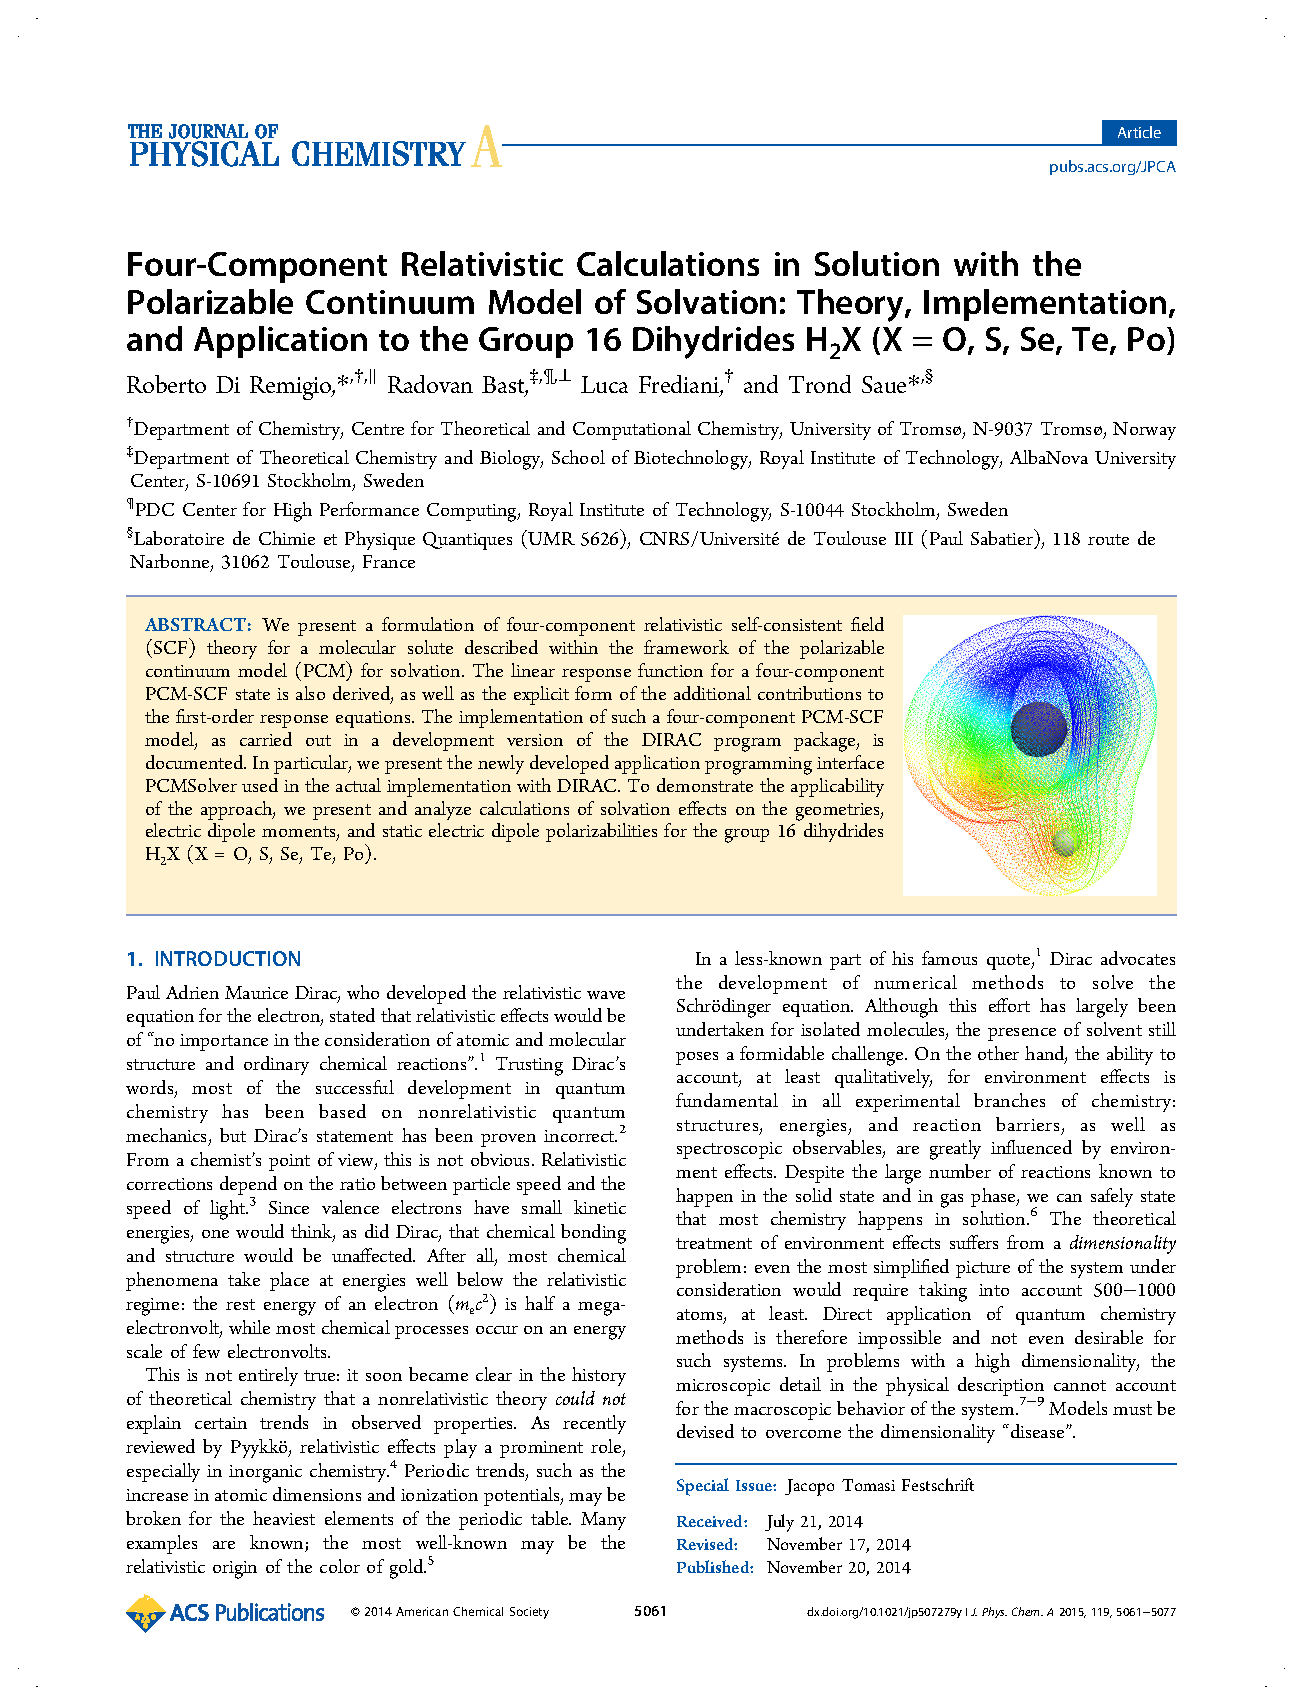
\includepdf[pages=-]{papers/relapcm.pdf}

\thispagestyle{empty}
\refstepcounter{dummy}
\addcontentsline{toc}{chapter}{\tocEntry{Paper II}}
%*******************************************************
\topskip0pt
\vspace*{\fill}
\begin{flushright}
{\Huge\paper{II}}
\end{flushright}

{\Large
\noindent\textsf{Wavelet Formulation of the Polarizable Continuum Model. II. Use of Piecewise
Bilinear Boundary Elements
}
\\
M. Bugeanu, \textbf{R. Di Remigio}, K. Mozgawa, S. S. Reine, H.
Harbrecht,  and L. Frediani
\\
\textit{Phys. Chem. Chem. Phys.}, \textrm{2015}, \textbf{17},
31566--31581
\\
DOI: \url{10.1039/C5CP03410H}
}
\vspace*{\fill}

\clearpage
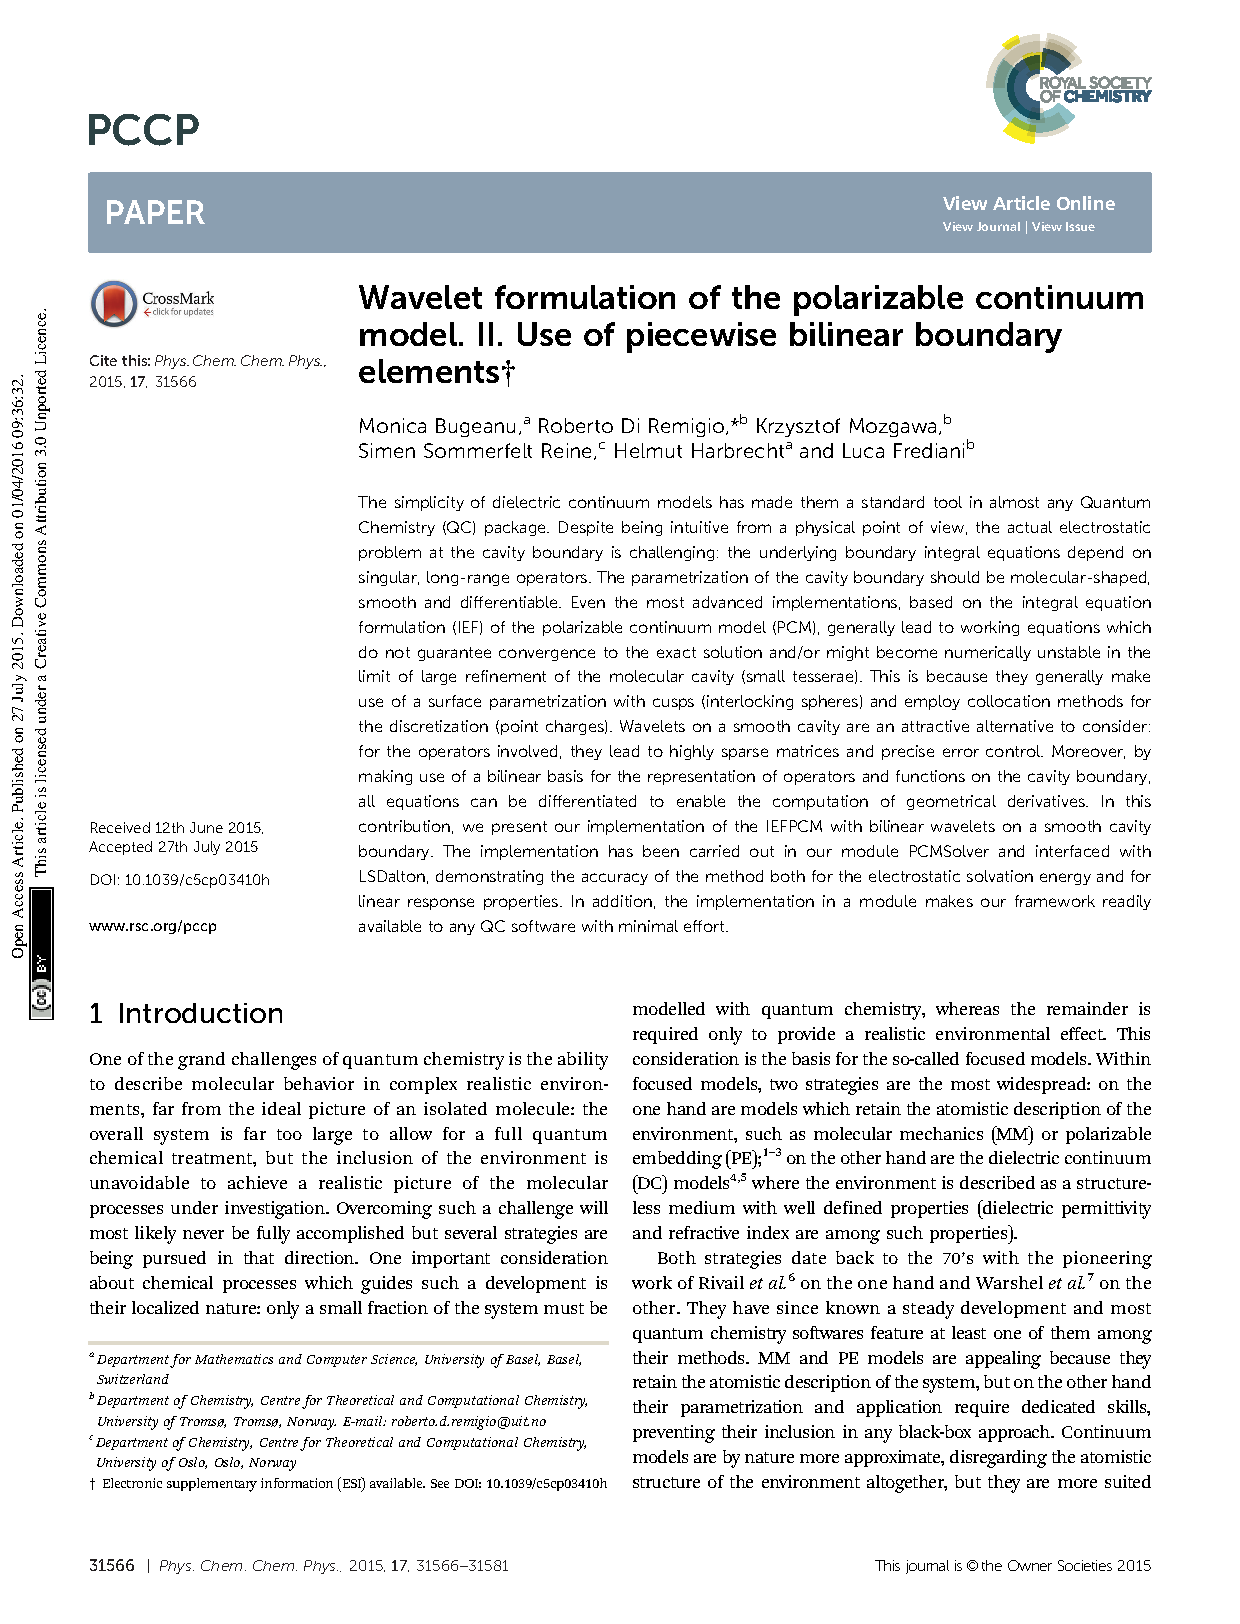
\includepdf[pages=-]{papers/wemlin.pdf}

\thispagestyle{empty}
\refstepcounter{dummy}
\addcontentsline{toc}{chapter}{\tocEntry{Paper III}}
%*******************************************************
\topskip0pt
\vspace*{\fill}
\begin{flushright}
{\Huge\paper{III}}
\end{flushright}

{\Large
\noindent\textsf{A Polarizable Continuum Model for Molecules at Spherical
Diffuse Interfaces
}
\\
    \textbf{R. Di Remigio}, K. Mozgawa, H. Cao, V. Weijo, and L.
    Frediani
\\
    \textit{J. Chem. Phys.}, \textrm{2016}, \textbf{144}, 124103
  \\
  DOI: \url{10.1063/1.4943782}
}
\vspace*{\fill}

\clearpage
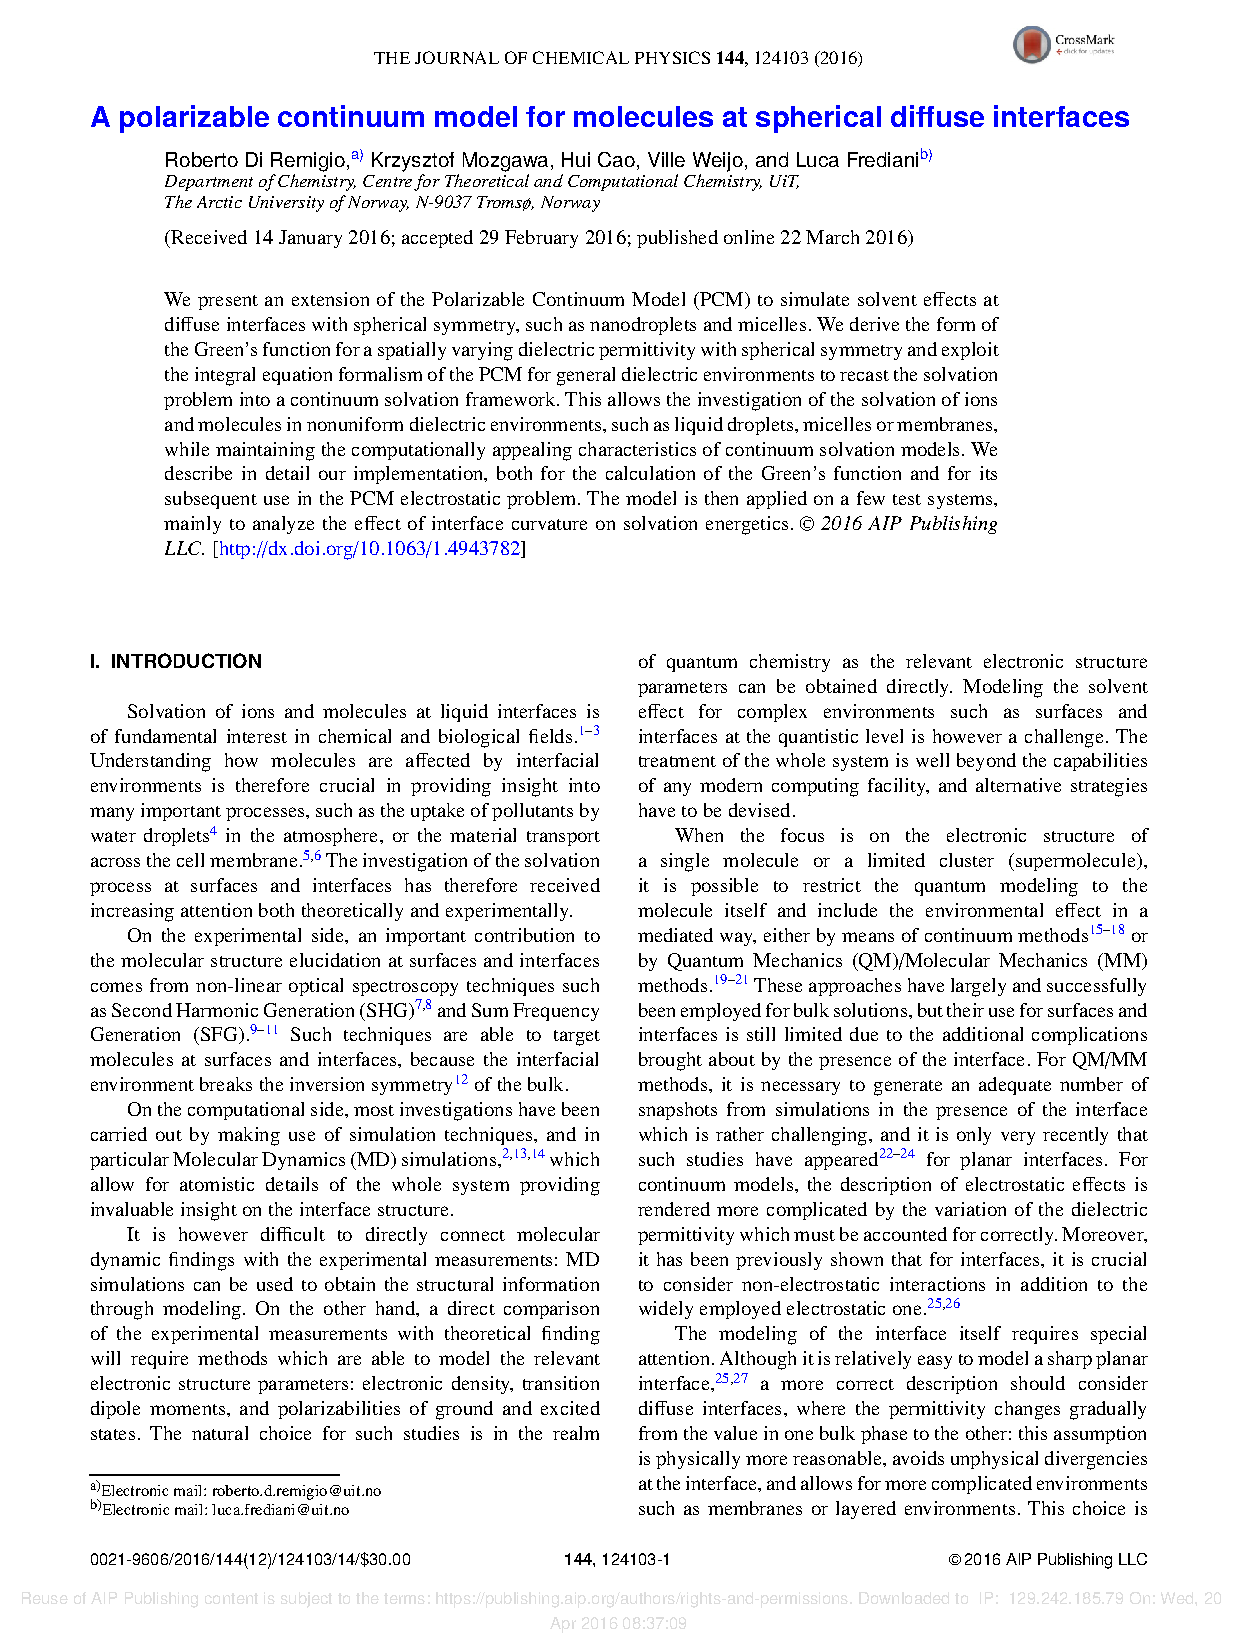
\includepdf[pages=-]{papers/spherical.pdf}

\thispagestyle{empty}
\refstepcounter{dummy}
\addcontentsline{toc}{chapter}{\tocEntry{Paper IV}}
%*******************************************************
\topskip0pt
\vspace*{\fill}
\begin{flushright}
{\Huge\paper{IV}}
\end{flushright}

{\Large
\noindent\textsf{Four-Component Relativistic Density Functional Theory with the
Polarizable Continuum Model: Application to EPR Parameters
and Paramagnetic NMR Shifts
}
\\
  \textbf{R. Di Remigio}, M. Repisky, S. Komorovsky, P. Hrobarik, L.
  Frediani, and K. Ruud
\\
  Accepted for publication in \textit{Mol. Phys.}
  \\
  DOI: \url{10.1080/00268976.2016.1239846}
}
\vspace*{\fill}

\clearpage
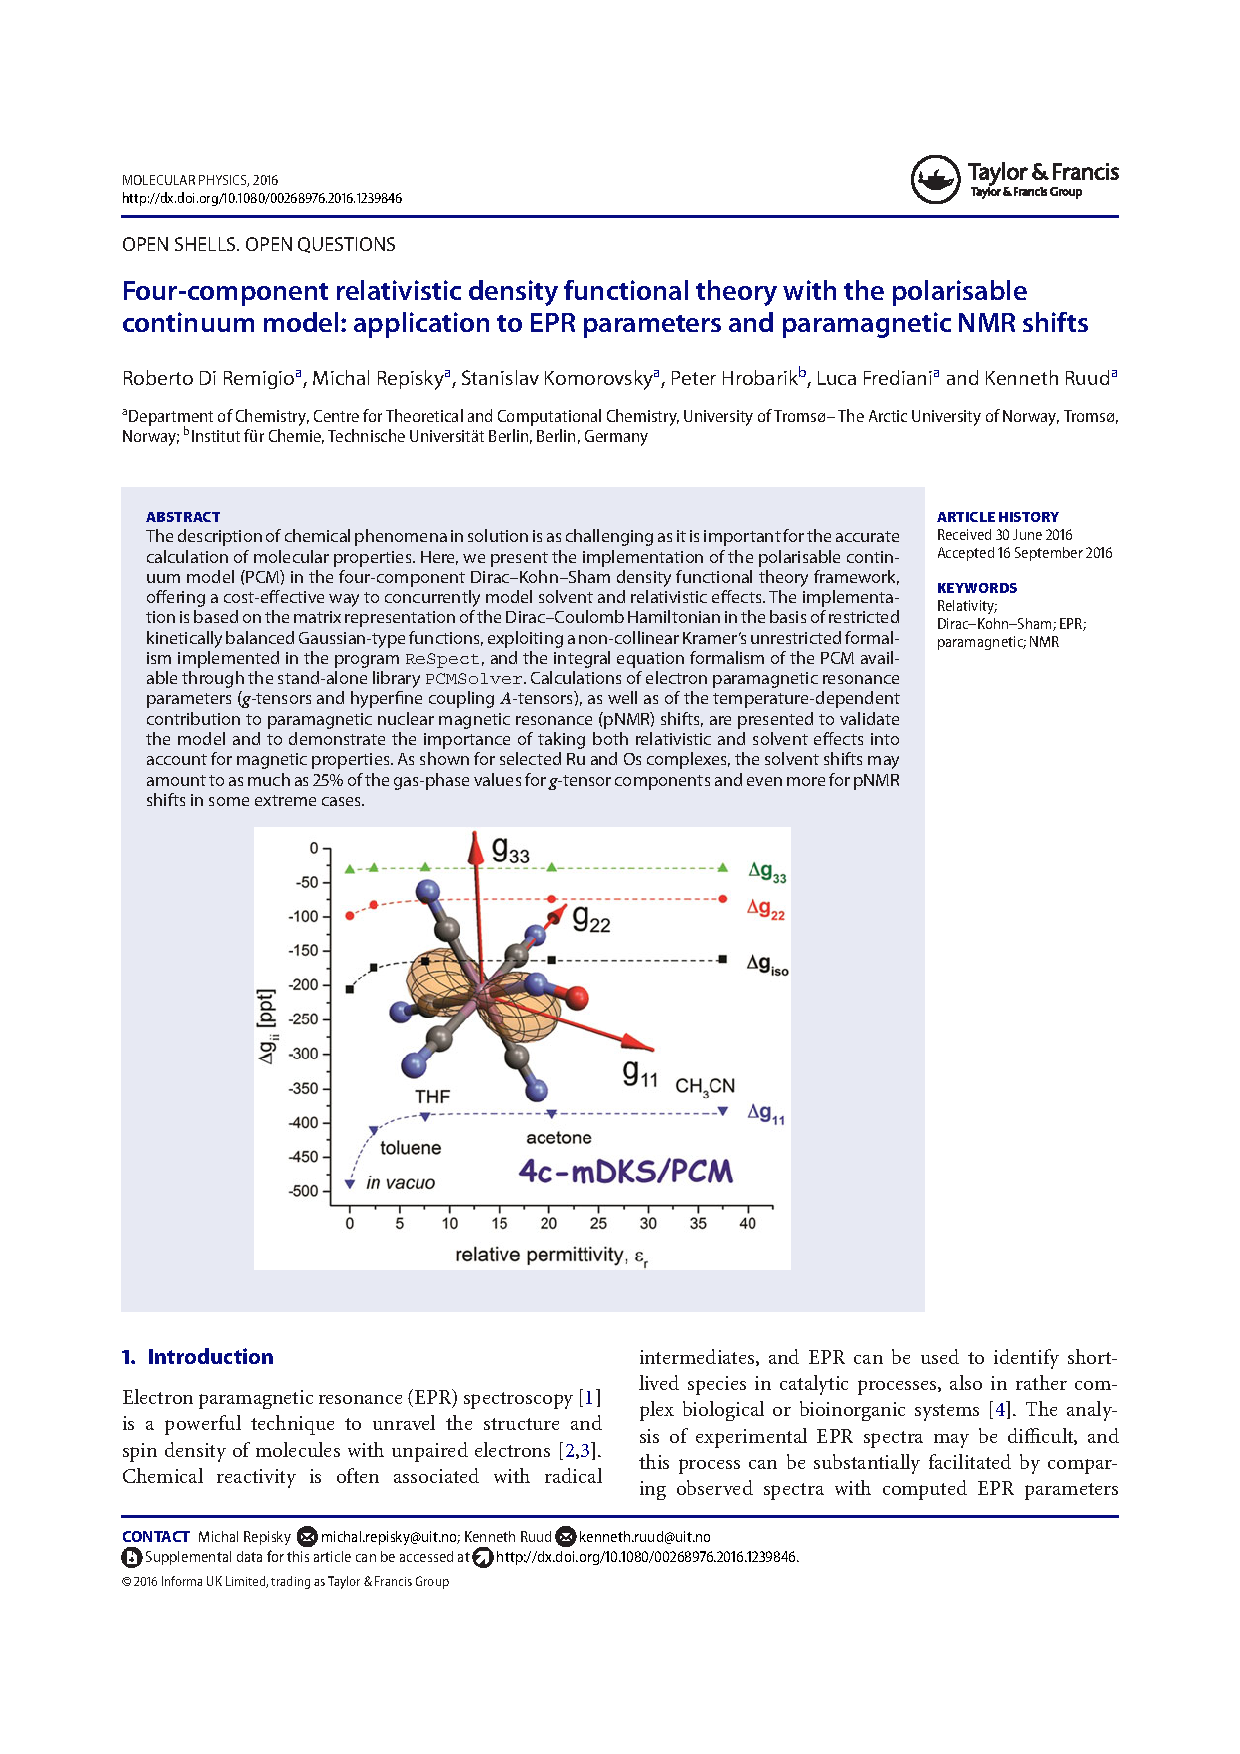
\includepdf[pages=-]{papers/pcmepr.pdf}
\pagebreak

\thispagestyle{empty}
\refstepcounter{dummy}
\addcontentsline{toc}{chapter}{\tocEntry{Paper V}}
%*******************************************************
\topskip0pt
\vspace*{\fill}
\begin{flushright}
{\Huge\paper{V}}
\end{flushright}

{\Large
\noindent\textsf{Open-Ended Formulation of Self-Consistent Field Response Theory with
the Polarizable Continuum Model for Solvation
}
\\
    \textbf{R. Di Remigio}, M. T. P. Beerepoot, Y. Cornaton, M. Ringholm,
    A. H. S. Steindal, K. Ruud, and L. Frediani
\\
    In preparation for submission to \textit{Phys. Chem. Chem. Phys.}
}
\vspace*{\fill}

\clearpage
%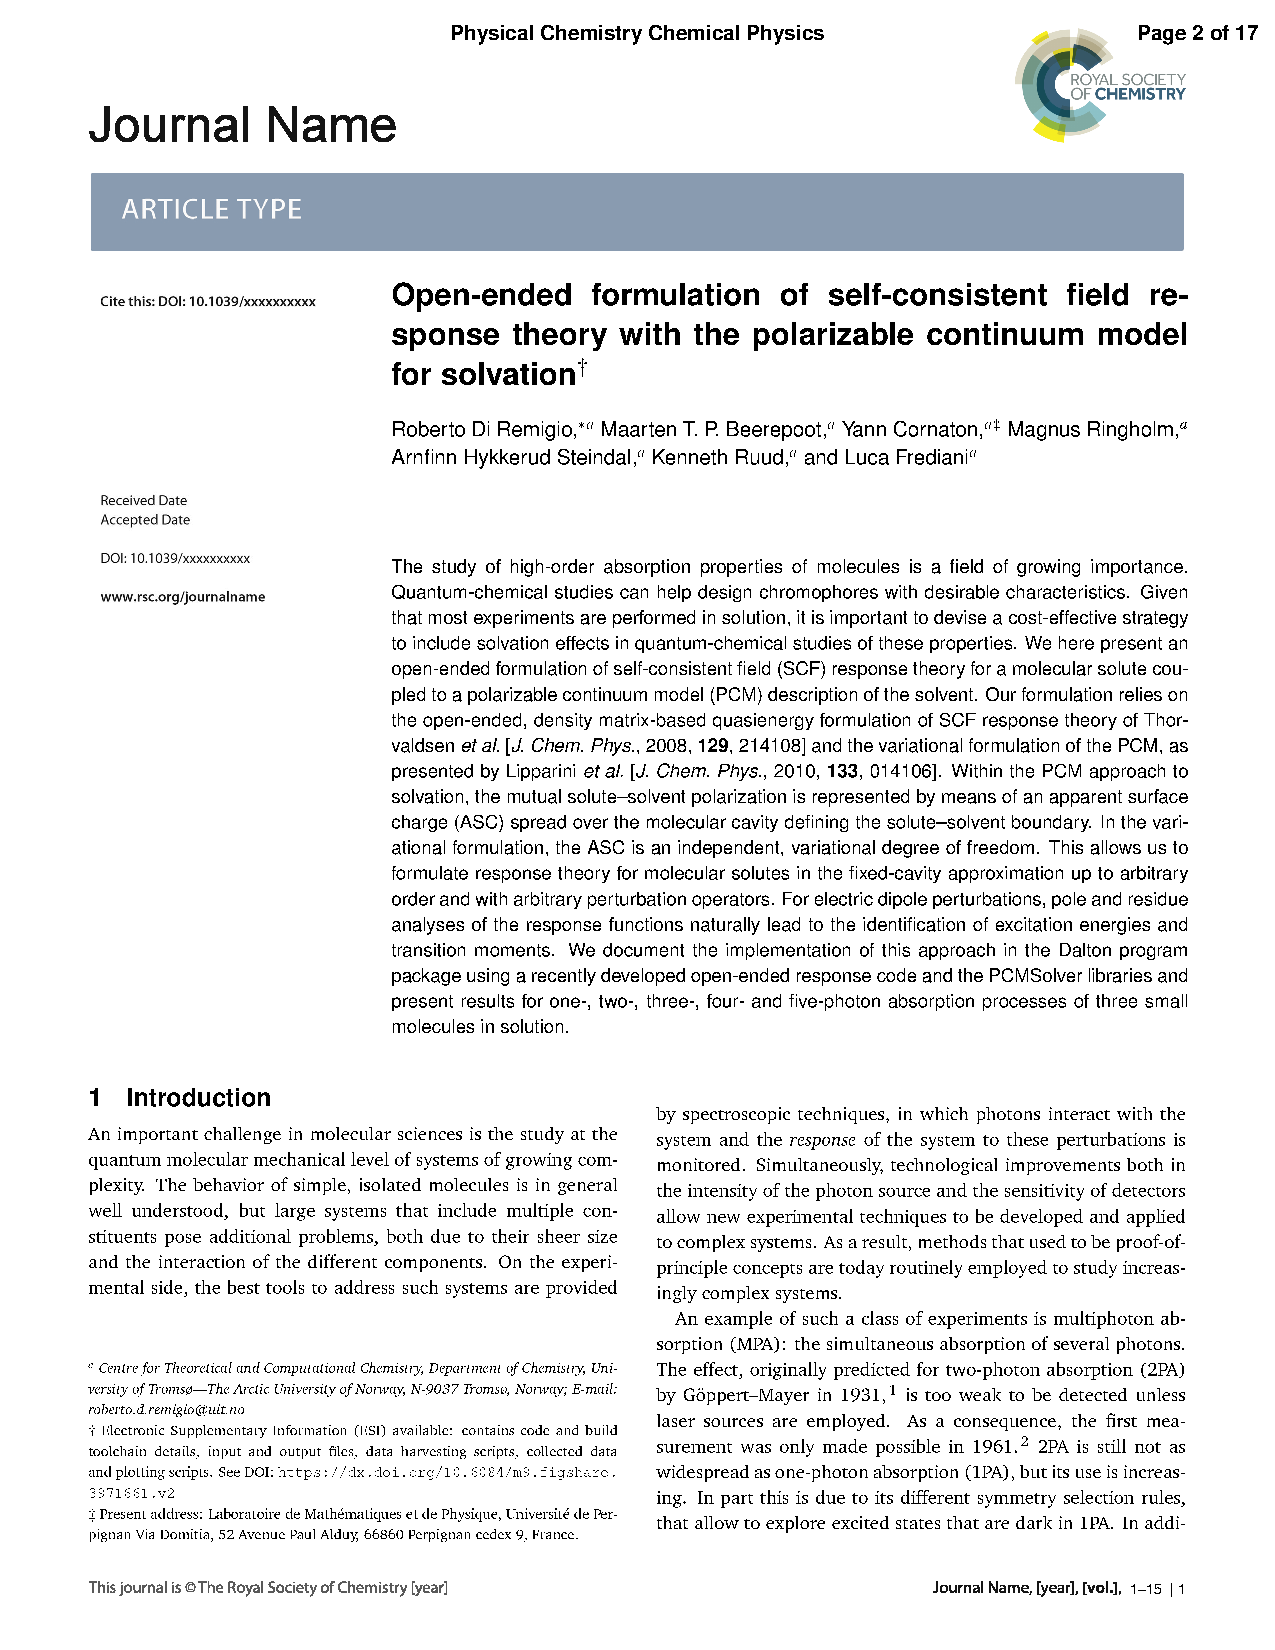
\includepdf[pages=-]{papers/pcmopenrsp.pdf}
\pagebreak
